% Milestone 7s (2026-11-18): the hull-ranking paper in IEEE conference format, for OCEANS (IEEE/MTS).
% Draft, not submitted. Every number is copied from ../experiments/results_*.txt (named in the
% text) via DRAFT.md; check_numbers.py checks each one against its file. Nothing new was run.
% Build: python3 make_figures.py && pdflatex main && bibtex main && pdflatex main && pdflatex main
\documentclass[conference]{IEEEtran}
\usepackage{amsmath,booktabs,tikz,url}
\usepackage[hidelinks]{hyperref}
\begin{document}
\title{Which Body Carries a Small Survey Payload Furthest per kWh?\\ A Swept Comparison of Seven Hull Types}
\author{\IEEEauthorblockN{Programme \texttt{marine-hull}}
\IEEEauthorblockA{Open research portfolio (MIT licensed); written with AI assistance (Claude Code).\\ Draft, not submitted.}}
\maketitle

\begin{abstract}
Small autonomous survey craft of 100 to 500\,kg are usually chosen for deck area and stability,
not endurance, and published comparisons fix one resistance method and one vehicle. We put seven
body types (monohull, catamaran, SWATH, planing hull, hydrofoil, buoyancy glider and propeller
AUV) on one energy basis, a 200\,kg craft with a 25\% battery mass fraction and a 30\,W payload,
and sweep every input we cannot source. Against a 4\,m Wigley-form monohull the catamaran
out-ranges it in 216 of 6{,}561 swept cases (3.3\%) and in none at equal length; SWATH, planing
and hydrofoil rungs win 0 of 4{,}374, 48 and 2{,}916. With form factors bounded by yacht-series
tank data the catamaran wins 0 of 6{,}561. The glider beats the AUV on energy per metre only
through hotel load: at equal hotel load it wins 0 of 2{,}430 cases, against vendor-implied AUV
loads it wins every case. The absolute range is not robust: hull-form constants together spread
best range by 20.6\%, and with deck solar the 5\,m craft makes about 133 to 69\,km/day from the
Equator to the Gulf of Alaska, each within about $\pm$10\%, with the site order unchanged in 500
of 500 draws. One published Wigley tank point says our swept form-factor box is conservative for
slender hulls. The ranking is the robust result; a buyer should measure hotel load before hull drag.
\end{abstract}

\section{Introduction}
If the payload's fixed power draw dominates at survey speed, the hull matters little; if not, it
matters a great deal. Surveys of unmanned surface vehicles catalogue hull types qualitatively
\cite{manley2008,liu2016}, and the regression in common use for resistance \cite{holtrop1982} was
fitted to ships of tens of metres, not to 3 to 5\,m craft. Nobody reports the region of inputs
where the answer changes.

We report that region. Contributions, stated narrowly: (i) a common energy-per-kilometre
comparison of seven body types with every unsourced input swept on a grid and every sourced one
named; (ii) the finding that the ranking is stable where the absolute range is not; (iii) a first
contact with tank data, one Wigley point and 308 yacht-series points, showing the swept form-factor
box is conservative for slender hulls and that Holtrop--Mennen over-predicts residuary resistance in
the survey regime; (iv) a seeded artefact with one command per table, stdlib Python only.

\section{Model}
\emph{Displacement hulls.} Frictional resistance from the ITTC 1957 line \cite{ittc1957} times a
form factor $(1+k)$, plus Michell thin-ship wave resistance \cite{michell1898} for Wigley hulls,
with Havelock two-hull interference for the catamaran and an interference factor swept over the
range measured by Insel and Molland \cite{insel1992,molland2011}. The wetted-surface constant
$c_s$ (2.6 to 3.4), the form factor (0.10 to 0.40) and a wave-term scale are swept.
\emph{Planing:} the Savitsky prismatic method \cite{savitsky1964}, without the mean-bottom-speed
correction. \emph{Hydrofoil:} Prandtl lifting line plus flat-plate struts, no ventilation
\cite{faltinsen2005}. \emph{Glider:} a steady glide at best-glide incidence with pump work
$B\tan\gamma/(2\eta)$ per metre, independent of dive depth \cite{rudnick2004,eriksen2001}; the AUV
is a same-mass, same-battery propeller body.

\emph{Range} is battery energy over $(P_{\mathrm{prop}}/\eta + P_{\mathrm{hotel}})$ times speed,
maximised over speed. At the best speed of a $v^3$ drag law the propulsive share of total power
is one third; the computed share is 0.33 to 0.37 over the hull box
(\texttt{results\_h1\_h5.txt}), so the best-range speed is set by the hotel load.
\emph{Deck solar} adds a daily mean harvest from NASA POWER insolation at five sites, with module
efficiency, temperature, soiling and electrical derates drawn jointly from their ranges.

\section{Results}
\subsection{Ranking against the monohull}
Table~\ref{tab:rank} compares each rung with the 4\,m Wigley monohull at its own best speed.
The monohull's best range is 560 to 1{,}188\,km (median 836\,km) at a median 1.05\,m/s in the
first sweep.

\begin{table}[t]
\caption{Rungs against the 4\,m Wigley monohull (200\,kg, 25\% battery, 30\,W hotel unless stated).}
\label{tab:rank}
\centering\footnotesize
\begin{tabular}{@{}lrl@{}}
\toprule
Rung & Cases & Wins over the monohull \\
\midrule
Catamaran (Michell + Havelock) & 6{,}561 & 216 (3.3\%); 0 of 2{,}187 equal length \\
Catamaran, tank-bound $k$ & 6{,}561 & 0 (ratio 0.74 to 0.97) \\
SWATH & 4{,}374 & 0 (ratio 0.552 to 0.826) \\
Planing (Savitsky) & 48 & 0 (ratio 0.055 to 0.138) \\
Hydrofoil, foilborne & 2{,}916 & 0 (ratio 0.064 to 0.248) \\
\midrule
Glider vs AUV, equal hotel & 2{,}430 & glider 0 \\
Glider vs REMUS-100-class AUV & 810 per row & glider longer in 100\% \\
\bottomrule
\end{tabular}
\end{table}

The catamaran's 216 wins all come from unequal lengths, and they rise with the monohull's form factor: its win
share is 0.0\%, 2.5\% and 7.4\% at monohull $k$ of 0.1, 0.25 and 0.4
(\texttt{results\_michell.txt}). With $k$ bounded to 0.03 to 0.15 for both hulls by the Delft
yacht-series tank data (Section~\ref{sec:tank}) it wins 0 of 6{,}561 (median range ratio 0.85,
max 0.97; \texttt{results\_lowk.txt}). With the Michell wave term in the same tank-bound box
(729 cases) it wins 7 (1.0\%) and 0 of 243 at equal length (ratio 0.73 to 1.02;
\texttt{results\_michell\_lowk.txt}); all 7 pair a 3\,m monohull with a longer catamaran at zero
interference, a length effect, not a hull-type effect. The prediction of no equal-length win was
logged before that run.

SWATH, planing and foil rungs lose at survey speed by wide margins (Table~\ref{tab:rank}); SWATH
still loses at a fixed 3\,m/s (median ratio 0.456; \texttt{results\_swath.txt}), and the foil's
best speed sits at the 10\,m/s grid ceiling in 369 of 1{,}620 feasible cases
(\texttt{results\_foil.txt}).

\subsection{Glider against propeller AUV}
At equal hotel load the AUV-over-glider energy-per-metre ratio has median 0.36 and the glider never
has the longer range; the glider ties when the AUV's hotel load is a median 4.87 times its own
(10th to 90th percentile 2.38 to 10.67; \texttt{results\_slocum.txt}). Against a REMUS-100-class
AUV whose non-propulsion load is implied by vendor endurance (107.3 to 170.3\,W of 125 to 188\,W
total), the glider is longer in every one of 810 cases per row (\texttt{results\_remus.txt}), at
about a tenth of the speed. The glider's edge is a hotel-load edge, so the proposal's hypothesis of
a speed crossover between 0.4 and 0.9\,m/s is refuted.

\subsection{What the ranking does not fix: absolute range}
With 27 combinations of $c_s$, $k$ and wave scale on one monohull, best range spans 763 to 921\,km
(20.6\%), though each constant alone moves it under 10\% ($c_s$ 9.0\%, $k$ 8.1\%, wave scale 0.8\%;
\texttt{results\_h1\_h5.txt}). Battery specific energy (150 to 250\,Wh/kg) swaps no pair in 2{,}187
cases, because range is linear in pack energy for every hull at fixed mass; only a fixed energy per
mission breaks that, and a catamaran-only overhead of 100\,Wh swaps 3 cases (0.1\%)
(\texttt{results\_h5\_overhead.txt}).

With deck solar, one-at-a-time sensitivity of km/day ranks hotel load ($-38.2$\% over 20 to
45\,W) above module efficiency ($+25.6$\%), derate ($+20.4$\%), $c_s$ ($-9.2$\%), form factor
($-8.2$\%) and wave scale ($-0.3$\%), while the best speed moves at most 0.2\,m/s
(\texttt{results\_solar\_sensitivity.txt}). Fig.~\ref{fig:solar} shows km/day with every power-side
input drawn jointly (500 draws): 133.4, 124.5, 97.2, 76.9 and 69.4\,km/day for the 5\,m craft from
the Equator to the Gulf of Alaska, each band within $-10$\%/$+9$\% of its median, and the site
order held in 500 of 500 draws (\texttt{results\_solar\_mc.txt}). The unsourced hull box adds
roughly another $\pm$10\% (\texttt{results\_solar\_hull\_uncertainty.txt}).

\begin{figure}[t]
\centering
% generated by make_figures.py from ../experiments/results_solar_mc.txt; do not edit
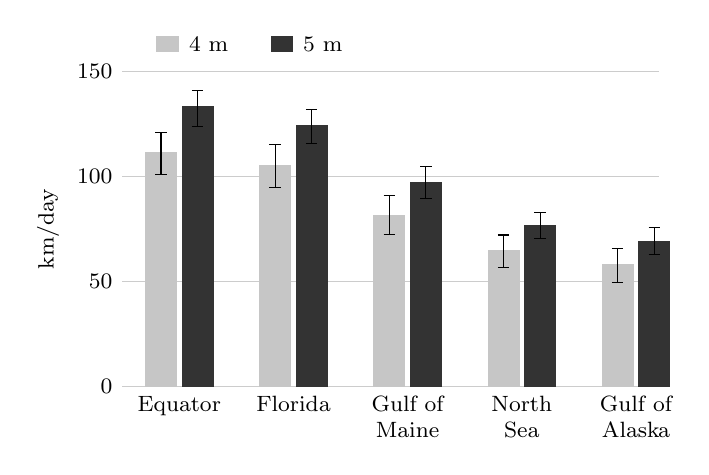
\begin{tikzpicture}[x=1.45cm,y=1cm,font=\footnotesize]
\draw[gray!40] (-0.1,0.000) -- (4.6,0.000);
\node[left] at (-0.1,0.000) {0};
\draw[gray!40] (-0.1,1.333) -- (4.6,1.333);
\node[left] at (-0.1,1.333) {50};
\draw[gray!40] (-0.1,2.667) -- (4.6,2.667);
\node[left] at (-0.1,2.667) {100};
\draw[gray!40] (-0.1,4.000) -- (4.6,4.000);
\node[left] at (-0.1,4.000) {150};
\node[rotate=90] at (-0.75,2.00) {km/day};
\fill[gray!45] (0.10,0) rectangle (0.38,2.973);
\draw (0.240,2.691) -- (0.240,3.221);
\draw (0.190,2.691) -- (0.290,2.691);
\draw (0.190,3.221) -- (0.290,3.221);
\fill[black!80] (0.42,0) rectangle (0.70,3.557);
\draw (0.560,3.304) -- (0.560,3.763);
\draw (0.510,3.304) -- (0.610,3.304);
\draw (0.510,3.763) -- (0.610,3.763);
\node[below,align=center] at (0.40,0) {Equator};
\fill[gray!45] (1.10,0) rectangle (1.38,2.813);
\draw (1.240,2.525) -- (1.240,3.069);
\draw (1.190,2.525) -- (1.290,2.525);
\draw (1.190,3.069) -- (1.290,3.069);
\fill[black!80] (1.42,0) rectangle (1.70,3.320);
\draw (1.560,3.085) -- (1.560,3.523);
\draw (1.510,3.085) -- (1.610,3.085);
\draw (1.510,3.523) -- (1.610,3.523);
\node[below,align=center] at (1.40,0) {Florida};
\fill[gray!45] (2.10,0) rectangle (2.38,2.184);
\draw (2.240,1.933) -- (2.240,2.421);
\draw (2.190,1.933) -- (2.290,1.933);
\draw (2.190,2.421) -- (2.290,2.421);
\fill[black!80] (2.42,0) rectangle (2.70,2.592);
\draw (2.560,2.384) -- (2.560,2.789);
\draw (2.510,2.384) -- (2.610,2.384);
\draw (2.510,2.789) -- (2.610,2.789);
\node[below,align=center] at (2.40,0) {Gulf of\\Maine};
\fill[gray!45] (3.10,0) rectangle (3.38,1.731);
\draw (3.240,1.515) -- (3.240,1.925);
\draw (3.190,1.515) -- (3.290,1.515);
\draw (3.190,1.925) -- (3.290,1.925);
\fill[black!80] (3.42,0) rectangle (3.70,2.051);
\draw (3.560,1.883) -- (3.560,2.211);
\draw (3.510,1.883) -- (3.610,1.883);
\draw (3.510,2.211) -- (3.610,2.211);
\node[below,align=center] at (3.40,0) {North\\Sea};
\fill[gray!45] (4.10,0) rectangle (4.38,1.552);
\draw (4.240,1.317) -- (4.240,1.752);
\draw (4.190,1.317) -- (4.290,1.317);
\draw (4.190,1.752) -- (4.290,1.752);
\fill[black!80] (4.42,0) rectangle (4.70,1.851);
\draw (4.560,1.675) -- (4.560,2.021);
\draw (4.510,1.675) -- (4.610,1.675);
\draw (4.510,2.021) -- (4.610,2.021);
\node[below,align=center] at (4.40,0) {Gulf of\\Alaska};
\fill[gray!45] (0.2,4.25) rectangle (0.4,4.45);
\node[right] at (0.4,4.35) {4 m};
\fill[black!80] (1.2,4.25) rectangle (1.4,4.45);
\node[right] at (1.4,4.35) {5 m};
\end{tikzpicture}

\caption{Deck-solar km/day of the 4\,m and 5\,m monohull at five NASA POWER sites: median of 500
joint draws of the power-side inputs, whiskers 5\% to 95\% (\texttt{results\_solar\_mc.txt};
drawn by \texttt{make\_figures.py}).}
\label{fig:solar}
\end{figure}

\section{Tank data}\label{sec:tank}
\emph{Wigley.} One published tank point, Ju (1983) at Froude number 0.267 on a 4\,m Wigley hull,
quoted by Wang et al.\ \cite{wang2017}, against Michell plus ITTC 1957: with no form factor the
model is within $-1$\% to +5\% of the measured $C_T = 4.16\times10^{-3}$ over 10 to 25\,$^\circ$C,
and the box's central $k=0.25$ is +18\% to +25\% high, so the swept box is conservative for
slender hulls (\texttt{results\_wigley\_tank.txt}). The implied $k$ is near zero: $-0.06$ to
$+0.01$ at this point, and a second laboratory's curve (Kajitani, via Ahmed et al.) gives $-0.04$ ($-0.13$ to $+0.05$) if its model is 1\,m long, a length we have not confirmed from the primary source.
One Froude number constrains $C_F(1+k)$ more than the wave model.

\emph{Holtrop--Mennen.} On the same point the 1982 method \cite{holtrop1982} is +19\% to +24\% high
with its own wetted-area regression and +33\% to +39\% with the true area
(\texttt{results\_holtrop.txt}); the excess is form factor and correlation allowance, not waves.
On 308 points of 22 Delft yacht-series hulls, at the survey Froude numbers 0.125 to 0.2 the method
over-predicts residuary resistance by a median 1.3 to 2.2 times in every swept case, an absolute gap
of about 0.4 per mille of weight at Fn 0.15, while at Fn 0.2 to 0.3 it is within 20\% for 42\% to
82\% of points (\texttt{results\_holtrop\_yacht.txt}). These are keeled sailing yachts read from a public mirror,
with midship and waterplane coefficients swept, so the result is exploratory.

\section{Threats to validity}
The hull constants are validated against one Wigley point, one 1\,m model and 22 keeled yacht hulls,
not against a resistance curve of a fuller, keel-less survey hull; that is the largest gap. Hotel-load,
module and glider sources are vendor sheets or abstracts, several read only as search excerpts.
Derate, soiling and temperature ranges are the authors' own, and are swept. There is no seakeeping
or stability; sea state enters only as a resistance multiplier, and a factor of 2 costs 21\% of
km/day while keeping the site order. The glider's range advantage is a persistence advantage: on
one 1.5\,kWh pack it covers 7 to 70 times the AUV's range in roughly 33 to 550 times the days
(\texttt{results\_endurance\_days.txt}), and in strong coastal currents it cannot hold its track.

\section{Conclusion}
For a 200\,kg, 4 to 5\,m survey craft the ranking of body types survives every unsourced input we
could sweep: the displacement monohull leads, and the catamaran wins only through unequal length or
an implausibly high monohull form factor. Absolute range does not survive: hull constants spread it
by a fifth and hotel load moves solar km/day more than any hull input. A buyer should measure the
payload's power draw before the hull's drag. Next: a slender survey-hull resistance curve below
Froude number 0.3 to test the form-factor bound, and the companion results on learned solar
corrections and wing-sail tack control, which are written up separately in the repository.

\bibliographystyle{IEEEtran}
\bibliography{refs}
\end{document}
